\subsection{Translation and Ribosomal Synthesis}
Lastly, we turn our attention to the process of synthesizing new proteins,
translation. This process stands as a good candidate for potentially limiting
growth since the synthesis of new proteins relies on the generation of
ribosomes, themselves proteinaceous molecules. As we will see in the coming
sections of this work, this poses a "chicken-or-the-egg" problem where the
synthesis of ribosomes requires ribosomes in the first place.

We will begin our exploration of protein translation in the same spirit as we
have in previous sections -- we will draw order-of-magnitude estimates based
on our intuition and available literature, and then compare these estimates
to the observed data. In doing so, we will estimate both the absolute number
of ribosomes necessary for replication of the proteome as well as the
synthesis of amino-acyl tRNAs. From there we consider the limitations on
ribosomal synthesis in light of our estimates on both the synthesis of
ribosomal proteins and our earlier results on rRNA synthesis.

\subsubsection{tRNA Synthetases}
We begin by first estimating the number of tRNA synthetases in \textit{E.
coli} needed to convert free amino-acids to polypeptide chains. Again using
an estimate of $\approx$ 3$\times$10$^6$ proteins per cell at a 5000 s
division time (BNID: 115702) and a typical protein length of $\approx$ 300
amino acids (BNID: 100017), we can estimate that a total of $\approx$ 10$^9$
amino acids are stitched together by peptide bonds.

How many tRNAs are needed to facilitate this remarkable number of amino acid
delivery events to the translating ribosomes? It is important to note that tRNAs
are recycled after they've passed through the ribosome and can be recharged with
a new amino acid, ready for another round of peptide bond formation. While some
\textit{in vitro} data exists on  the turnover of tRNA in \textit{E. coli} for
different  amino acids, we can make a reasonable estimate by comparing the
number of amino acids to be  polymerized to cell division time. Using our
stopwatch of 5000 s and 10$^9$ amino acids, we arrive at a requirement of
$\approx$ 2 $\times$ 10$^5$ tRNA molecules to be consumed by the ribosome per
second.

There are many processes which go into synthesizing a tRNA and ligating it
with the appropriate amino acids. As we discussed previously, there appear to
be more than enough RNA polymerases per cell to synthesize the needed pool of
tRNAs. Without considering the many ways in which amino acids can be
scavenged or synthesized \textit{de novo}, we can explore ligation as a
potential rate limiting step. The enzymes which link the correct amino acid
to the tRNA, known as tRNA synthetases or tRNA ligases, are incredible in
their proofreading of substrates with the incorrect amino acid being ligated
once out of every $10^4$ to $10^5$ events (BNID: 103469).
This is due in part to the consumption of energy as well as a multi-step
pathway to ligation. While the rate at which tRNA is ligated is highly
dependent on the identity of the amino acid, it is reasonable to state that
the typical tRNA synthetase has charging rate of $\approx$ 20 AA per tRNA
synthetase per second (BNID: 105279).

We can make an assumption that amino-acyl tRNAs are in steady-state where they
are produced at the same rate they are consumed, meaning that $2 \times 10^5$
tRNAs must be charged per second. Combining these estimates together, as shown schematically
in \FIG{protein_synthesis}(A), yields an estimate of $\sim$ 10$^4$ tRNA
synthetases per cell with a division time of 5000 s. This point estimate is in
very close agreement with the observed number of synthetases (the sum of all 20
tRNA synthetases in \textit{E. coli}). This estimation strategy seems to
adequately describe the observed growth rate dependence of the tRNA synthetase copy
number (shown as the grey line in \FIG{protein_synthesis}(B)), suggesting that
the copy number scales with the cell size.

In total, the estimated and observed $\sim$ 10$^4$ tRNA synthetases occupy
only a meager fraction of the total cell proteome, around 0.5\% by abundance. It
is reasonable to assume that if tRNA charging was a rate limiting process, cells
would be able to increase their growth rate by devoting more cellular resources
to making more tRNA synthases. As the synthesis of tRNAs and the corresponding
charging can be highly parallelized, we can argue that tRNA charging is not a
rate limiting step in cell division, at least for the growth conditions explored
in this work.

\subsubsection{Protein Synthesis}
With the number of tRNA synthetases accounted for, we now consider the abundance
of the protein synthesis machines themselves, ribosomes. Ribosomes are enormous
protein/rRNA complexes that facilitate the peptide bond formation between amino
acids in the correct sequence as defined by the coding mRNA. Before we examine
the synthesis of the ribosome proteins and the limits that may place on the
observed bacterial growth rates, let's consider replication of the cellular
proteome.

While the rate at which ribosomes translate is known to have a growth
rate dependence \cite{dai2018}, for the purposes of our order-of-magnitude
estimate we make the approximation that translation occurs at a rate of
$\approx$ 15 amino acids per second per ribosome (BNID: 100233). Under this
approximation and assuming a division time of 5000 s, we can arrive at an
estimate of $\approx 10^4$ ribosomes are needed to replicate the cellular
proteome, shown in \FIG{protein_synthesis}(B). This point estimate, while
glossing over important details such as chromosome copy number and
growth-rate dependent translation rates, proves to be notably accurate when
compared to the experimental observations (\FIG{protein_synthesis}(B)).

\begin{figure}
    \begin{fullwidth}
    \centering{
        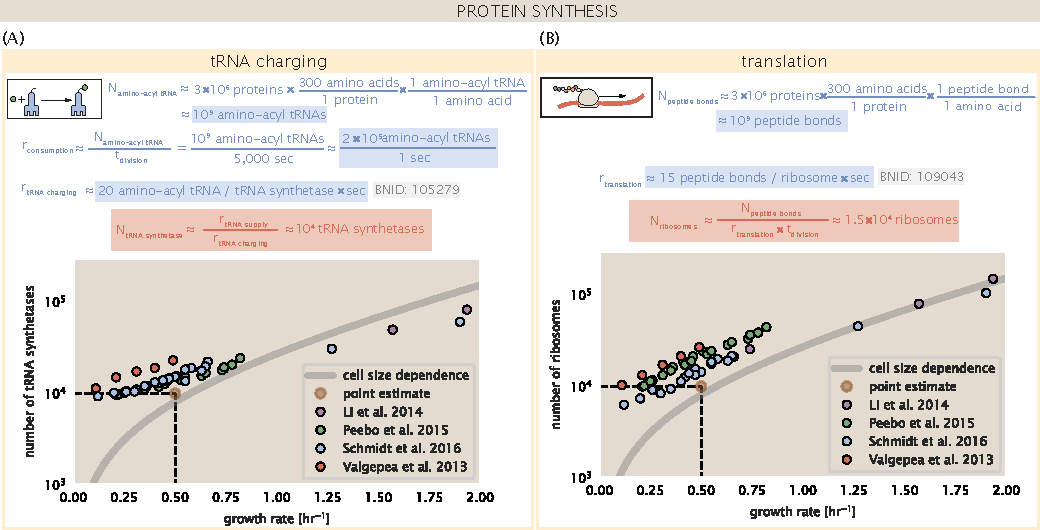
\includegraphics{main_figs/fig8_protein_synthesis.pdf}
        \caption{\textbf{Estimation of the required tRNA synthetases and
        ribosomes.} (A) Estimate for the
        number of tRNA synthetases that will supply the required amino acid
        demand. The sum of all tRNA synthetases copy numbers are plotted as a
        function of growth rate ([ArgS], [CysS], [GlnS], [GltX], [IleS], [LeuS],
        [ValS], [AlaS]$_2$, [AsnS]$_2$, [AspS]$_2$, [TyrS]$_2$, [TrpS]$_2$,
        [ThrS]$_2$, [SerS]$_2$, [ProS]$_2$, [PheS]$_2$[PheT]$_2$, [MetG]$_2$,
        [lysS]$_2$, [HisS]$_2$, [GlyS]$_2$[GlyQ]$_2$). (B) Estimate of the
        number of ribosomes required to synthesize 10$^9$ peptide bonds with an
        elongation rate of 15 peptide bonds per second. The
        average abundance of ribosomes is plotted as a function of growth rate.
        Our estimated values are shown for a growth rate of 0.5 hr$^{-1}$.
        Grey lines correspond to the estimated complex abundance calculated at
        different growth rates. See Appendix \nameref{sec:SI_continuum_est} for a more
        detail description of this calculation.}
    \label{fig:protein_synthesis}
    }
    \end{fullwidth}
\end{figure}
